%!TEX root = ../sbc-template.tex

O processo de classificação indicativa integra o sistema de garantias dos direitos da criança e do adolescente quanto a promover, defender e garantir o acesso a espetáculos e diversões públicas adequados à condição de seu desenvolvimento, mas reserva-se o direito final aos pais e responsáveis quanto à escolha do conteúdo adequado a estes\cite{eca}.

No Brasil, a \emph{Coordenação de Classificação Indicativa} (Cocind), vinculada ao Ministério da Justiça, é o órgão responsável pela classificação indicativa de obras destinadas à televisão e outros meios, incluindo até mesmo aplicativos. A análise da classificação indicativa realizada pelo Cocind considera o grau de incidência de conteúdos de sexo e nudez, violência e drogas nas obras a serem avaliadas, como sintetizado na Tabela \ref{tab:categorias}. O processo envolve o exame do conteúdo das obras a serem classificadas, a atribuição de classificação indicativa, verificação do cumprimento das normas associadas e advertência por descumprimento destas normas \cite{portaria:ci}.


%!TEX root = ../../novoIndex.tex
\begin{table}[!ht]
  \scalefont{0.8}
  \caption{Categorias de classificação indicativa propostas pela Portaria No. 368, de 11 de Fevereiro de 2014. Fonte: \cite{ci:guia}}
  \label{tab:categorias}
	\centering
	\begin{tabular}{p{4cm} p{1.5cm} p{8cm}}
		\hline
		\textbf{Categoria} & \textbf{Símbolo} & \textbf{Descrição do Conteúdo} \\
		\hline
		Livre & \vfill
\includegraphics[width=0.05\textwidth]{img/livre.png} \vfill&
				Conteúdo predominantemente positivo ou que contem imagens de violência fantasiosa, armas sem violência, mortes sem violência, ossadas e esqueletos sem violência, nudez não erótica e consumo moderado ou inusitado de drogas lícitas. \\
		\hline
		Não recomendado para menores de dez anos &\vfill 
\includegraphics[width=0.05\textwidth]{img/10anos.png}\vfill &
		 		Presença de armas com violência; medo ou tensão; angústia; ossadas e esqueletos com resquícios de ato de violência; atos criminosos sem violência; linguagem depreciativa; conteúdos educativos sobre sexo; descrições verbais do consumo de drogas lícitas; discussão sobre o tráfico de drogas; e o uso medicinal de drogas ilícitas.\\
		\hline
		Não recomendado para menores de doze anos &\vfill 
\includegraphics[width=0.05\textwidth]{img/12anos.png}\vfill &
				Ato violento; lesão corporal; descrição de violência; presença de sangue; sofrimento da vítima; morte natural ou acidental com violência; ato violento contra animais; exposição ao perigo; exposição de pessoas em situações constrangedoras ou degradantes; agressão verbal; obscenidade; \emph{bullying}; exposição de cadáver; assédio sexual; supervalorização de beleza física; supervalorização do consumo; nudez velada; insinuação sexual; carícias sexuais; masturbação não explícita; linguagem chula; linguagem de conteúdo sexual; simulações de sexo; apelo sexual; consumo de drogas lícitas; indução ao uso de drogas lícitas; consumo irregular de medicamentos; menção a drogas ilícitas.\\
		\hline
		Não recomendado para menores de catorze anos &\vfill 
\includegraphics[width=0.05\textwidth]{img/14anos.png}\vfill &
				Morte intencional; estigma ou preconceito; nudez; erotização; vulgaridade; relação sexual não explícita; prostituição; insinuação do consumo de drogas ilícitas; descrições verbais do 	consumo de drogas ilícitas; e discussão sobre a descriminalização de drogas ilícitas.\\
		\hline
		Não recomendado para menores de dezesseis anos &\vfill 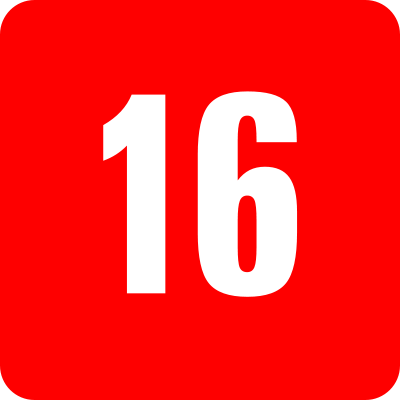
\includegraphics[width=0.05\textwidth]{img/16anos.png}\vfill &
				Estupro; exploração sexual; coação sexual; tortura; mutilação; suicídio; violência gratuita ou banalização da violência aborto, pena de morte ou eutanásia; relação sexual intensa não explícita; produção ou tráfico de qualquer droga ilícita, consumo de drogas ilícitas; indução ao consumo de drogas ilícitas.\\
		\hline
		Não recomendado para menores de dezoito anos &\vfill 
\includegraphics[width=0.05\textwidth]{img/18anos.png}\vfill &
				Violência de forte impacto; elogio, glamourização e/ou apologia à violência; crueldade; crimes de ódio; pedofilia; sexo explícito; situações sexuais complexas ou de forte impacto; apologia ao uso de drogas ilícitas.\\
		\hline
	\end{tabular}
\end{table}


No mundo, conteúdos televisivos são comumente classificados quanto ao grau de incidência de assuntos como linguagem vulgar, conteúdo sexual, drogas e violências, além de temas como conteúdo perturbador e discriminação, a exemplo dos Países Baixos. É frequente a aplicação de restrições de horários para a transmissão de conteúdos restritivos. As classes podem incluir restrição de idade e/ou supervisão de responsáveis, como ocorre nos Estados Unidos, Chile, Equador, Hong Kong, entre outros. Em países como a Austrália e Nova Zelândia, há um sistema de classificação indicativa para televisão aberta e outro para fechada, e um sistema de classificação especial para programas direcionados ao público infantil, na Austrália. Na Colômbia, é proibida a transmissão aérea de pornografia, mesmo em canais adultos. O ícone da classificação indicativa frequentemente deve ser exibido antes do início do programa, antes do início de cada bloco, a exemplo do Brasil, ou durante toda a transmissão do programa, como é o caso da França.  Na Alemanha, apenas o aviso ``O programa a seguir não é recomendado para espectadores abaixo de 16/18 anos'' é mostrado na tela caso haja conteúdo potencialmente ofensivo. Em países como Portugal, Polônia e Singapura, a implantação de sistemas de classificação indicativa é recente, posterior ao ano 2000. \todo{Falta referência}
